\documentclass[12pt, letterpaper]{article}
\usepackage[utf8]{inputenc}
\usepackage{indentfirst}
\usepackage{graphicx}
\usepackage{setspace}
\usepackage[numbers]{natbib}
\usepackage [autostyle, english = american]{csquotes}
\MakeOuterQuote{"}
\usepackage{layout}
\usepackage[title]{appendix}
\usepackage[justification=centering]{caption}
\usepackage{titlesec}


\begin{document}

\setcounter{secnumdepth}{-1}
\titlespacing*{\section}{0pt}{2\baselineskip}{.33333\baselineskip}

%Cover page: 5pts
\title{MA348 Numerical Analysis, Numerical Error in Computing Systems}
\author{David Jefts}
\date{January 25th, 2019}
\begin{titlepage}
	\centering
	\maketitle
	\centering
	\hfill
	\vfill
\end{titlepage}

\setlength{\voffset}{-0.5in}
\setlength{\headsep}{10pt}

%Introduction: 5pts
%Describe the problem and state objectives
\section{Introduction}
	The goal of this lab is to represent error in computers due to truncation and the limits of the mantissa-exponent form of number representation. This lab uses the function $f(x)=-0.1x^4-0.15x^3-0.5x^2-0.25x+1.2$ as the base function for demonstration purposes. The code used in this lab estimates the derivative of this base function using the second order approximation function, $f'(x)\approx\frac{f(x+h)-f(x-h)}{2h}$, to show how the error changes as you decrease $h$. The $x$ value for this activity is $0.5$

%Theory-Analysis: 5pts
%State assumptions and develop equations
\section{Theory-Analysis}
	This report assumes that computers have a limited way to represent numbers, therefor causing truncation and round-off errors. In the operating system utilized by the author, the computer stores each number with 64 bits of memory, leading to errors when the numbers used require more bits to be properly represented. The function $f(x)$ was given in the original lab activity, and the derivative function is a finite quotient function that normally is written as a limit, where $h$ approaches $0$. However, in this scenario the limit is represented by the steadily decreasing $h$ used in the code. Additionally, each iteration uses a fixed, non-zero value for $h$. 

%Numerical Solution: 20pts
%Describe the numerical methods used to solve the problem
\section{Numerical Solution}
	This problem was solved using Fortran code and the second order approximation function for a first derivative function to iteratively find the value of $f'(0.5)$. Each iteration decreased the value of $h$ by $\frac{1}{10}$ and then calculated the error as compared to a hand-calculated "true" value of $f'(0.5)=-0.9125$. gnu-plot was used to plot the graphs shown in the appendices and used for conclusions.

%Results and Discussion: 45pts
%Tabulate and plot the results, compare results, and discuss the accuracy of results
\section{Results and Discussion}
	The graph in Appendix A shows a plot of the step size vs the error, with step size increasing logarithmically from $10^{-10}$ to $10^{-1}$. Note that both axis are on a logarithmic scale to help visualize the error change better. A tabular version of the data can be found below as well.
	
	\begin{table}[h]
		\centering
		\begin{tabular}{|l|l|}
			\hline
    			\textbf{Step Size $(h)$} & \textbf{True Error $(\varepsilon)$} \\ \hline
			1 & 0.35 \\ \hline
			0.1 & 0.00349998 \\ \hline
			0.01 & 0.0000349814 \\ \hline
			0.001 & 0.000000331374 \\ \hline
			0.0001 & 0.0000000151267 \\ \hline
			1.00E-05 & 0.0000000185962 \\ \hline
			1.00E-06 & 0.0000000186184 \\ \hline
			1.00E-07 & 0.0000000188404 \\ \hline
			1.00E-08 & 0.0000000149547 \\ \hline
			1.00E-09 & 0.00000000385242 \\ \hline
			1.00E-10 & 0.00000005165870 \\ \hline
		\end{tabular}
		\centering
		\caption{Table of values for the derivative of the function $f(x)=-0.1x^4-0.15x^3-0.5x^2-0.25x+1.2$}
		\label{fig:table}
	\end{table}
	
	As shown, the error reaches a minima when the step size is around $1^{-9}$ because the second order approximation function is divided by the step size $(h)$. The nature of the function means that eventually the error will "switch" from truncation error to rounding error when the numbers are too small for the computer to be able to store and represent them properly.
	
%Conclusions: 20pts
%Comment on the efficiency of the solvers
\section{Conclusions}
	The solver worked fairly efficiently, reaching a minimum error after only 10 iterations. The code itself could be optimized by ending the program if the error begins to increase significantly. It is fairly surprising, at least to me, is that the computer appears to only properly represent numbers greater than $10^{-10}$.  Additionally, after converting both axes on the graph to logarithmic the graph appears to have a weird "hump" between the $h$ values of $1^{-8}$ and $1^{-4}$.

\pagebreak

%Appendices
%Include listings of the source codes, include printed copies of the output files
\appendix
	\section{Appendix A}
		\begin{figure}[h]
			\centering
			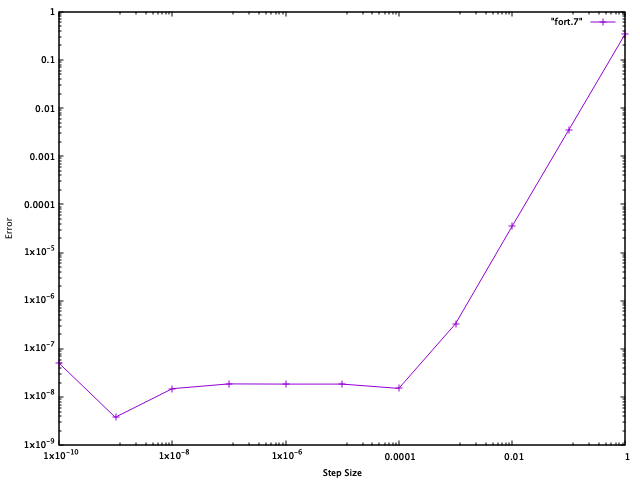
\includegraphics[width=\linewidth]{StepVsErrorGraph.png}
			\caption{Graph of step-size vs error}
			\label{fig:graph}
		\end{figure}
	\pagebreak
	
	\section{Appendix B}
		\begin{figure}[h]
			\centering
			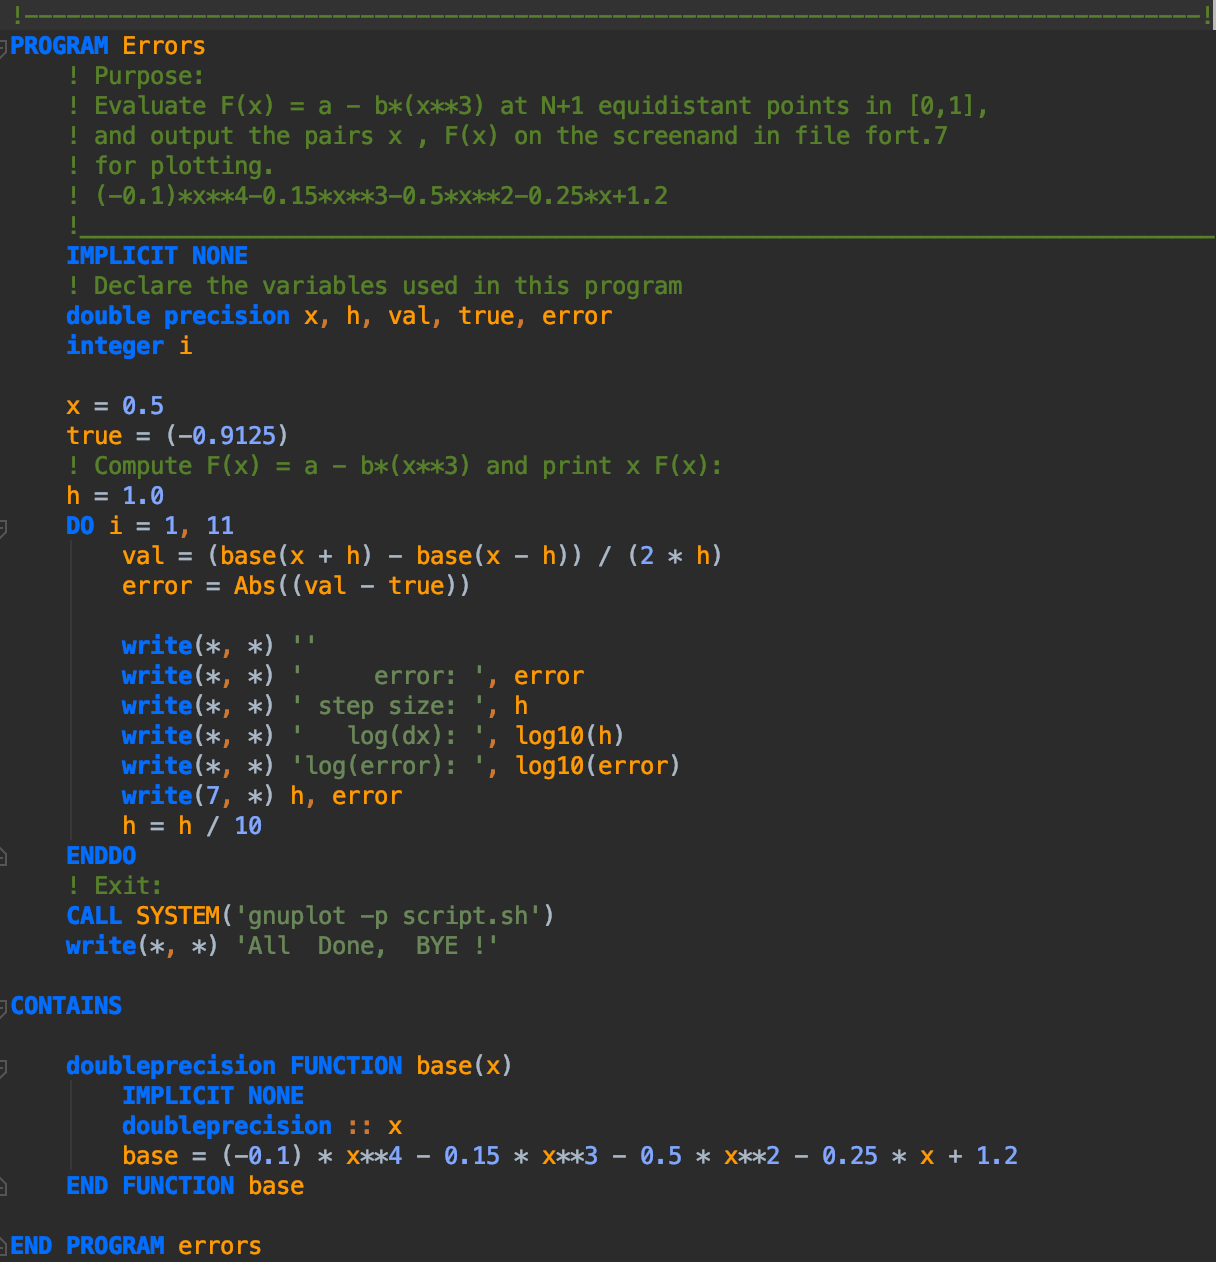
\includegraphics[width=.988975\linewidth]{FortranCode.png}
			\caption{Fortran program code}
		\end{figure}
		
		\begin{figure}[h]
			\centering
			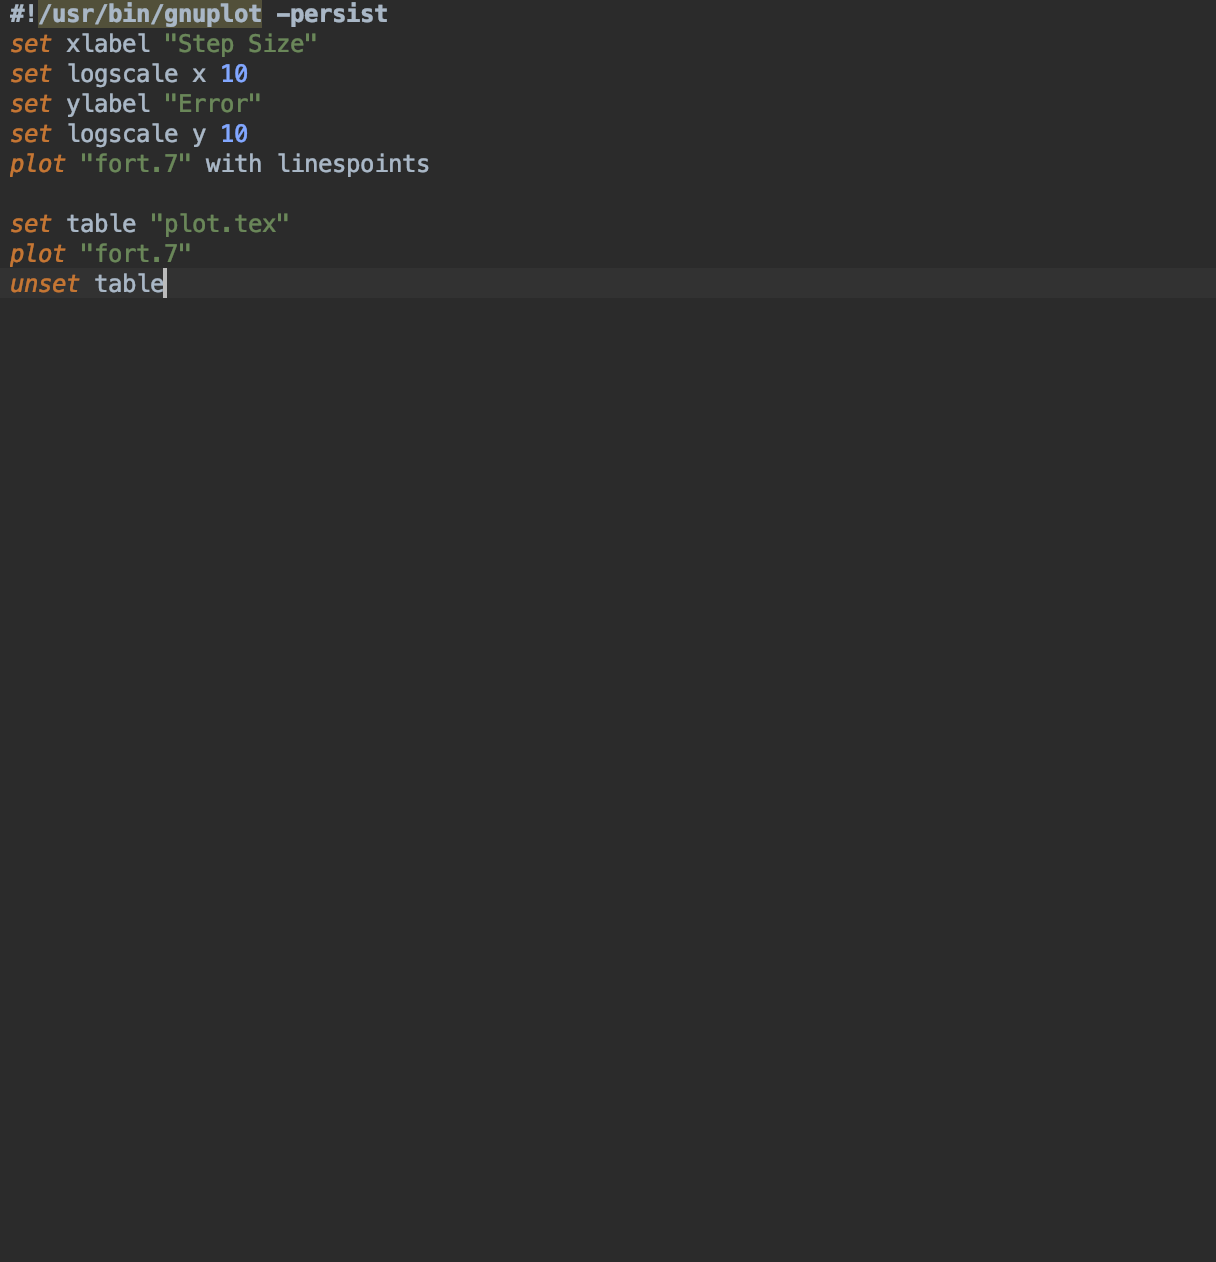
\includegraphics[width=\linewidth]{GnuplotCode.png}
			\caption{Script for gnuplot to set up the graph correctly}
		\end{figure}


\end{document}
